\chapter{Nástroj pro tvorbu jazyků}

V této kapitole budou popsány typy jazyků a nástroj pro jejich tvorbu. Budou zde popsány \textit{doménově specifické jazyky}, \textit{jazyky pro obecné použití} a nástroj Xtext.

\section{GPL a DSL}

Programovací jazyky jsou nástrojem člověka, pomocí kterého dokáže sdělit počítači požadavky, které vykonávat. Programovací jsou různé a mají různá zaměření a funkce. Hlavními dvěma typy jsou \textit{doménově specifické jazyky} a \textit{jazyky pro obecné použití}. Tyto dva typy budou popsány v následujících částech. 

\subsection{GPL}

\textit{Jazyk pro obecné použití} (z angl. \textit{General-Purpose Language}) (GPL) je programovací jazyk používaný pro řešení veškerých libovolně složitých problémů. Těmito jazyky je většina známých a používaných jazyků. Příkladem mohou být jazyky \textit{C}, \textit{C++}, \textit{C\#}, \textit{Java}, \textit{PHP}, \textit{BASIC}, \textit{Assembler}, \textit{Python} a mnoho dalších. Platí, že každý jazyk je vhodný pro jiné platformy, nebo typy problémů, ale pomocí všech bychom měli být schopni vyřešit libovolný problém.

Jednotlivé jazyky také rozlišujeme podle jejich úrovně. Nízkoúrovňové jazyky vyžadují přímou práci s pamětí počítače, kde proměnné a jiné struktury alokujeme na přesné místo v paměti. Takovými jazyky jsou například jazyky \textit{C}, \textit{BASIC} a další.

Krom nízkoúrovňových jazyků existují i vysokoúrovňové jazyky. Takové jazyky mají práci s pamětí již implementovanou u svého překladu a není vyžadována po programátorovi, který jazyk využívá. Také obsahují velké množství datových struktur, které by si programátor musel vytvořit v nízkoúrovňovém jazyce sám. Takovými strukturami mohou být různé typy listů, hashmapy, nebo objekty. Takovými jazyky jsou například jazyky \textit{C\#} nebo \textit{Java}.

\subsection{DSL}

\textit{Doménově specifické jazyky} (z angl. \textit{Domain-Specific Language}) (DSL) jsou jazyky, které jsou určené k přímému popisu nějaké domény. Dle \cite{Xtext} je hlavní myšlenkou mít koncept a zápis co nejblíže reálnému problému v dané doméně.

Autoři uvádějí problém ze života, kde chceme z jablka odstranit jádro. GPL přirovnávají k noži, kterým jsme schopni tento proces uskutečnit, avšak je vhodný pouze pokud ho neděláme často. Ale pokud tento problém řešíme frekventovaně, je lepší použít vykrajovač jablek, v tomto případě DSL. 

Dle autorů \cite{Xtext} existuje několik velmi známých doménově specifických jazyků. Jedním z nich je například jazyk \textit{SQL}, který se zaměřuje na dotazování relačních databází. Dalším příkladem mohou být regulární výrazy nebo například jazyky poskytované nástroji jako je \textit{MathLab}. Také většina jazyků postavených na jazyce XML jsou doménově specifické. Účelem XML je umožnit jednoduché tvoření nových jazyků. Bohužel XML používá pevnou konkrétní syntaxi, což může být složité a nečitelné lidmi. 

Dle \cite{Fowler} dělíme DSL na interní a externí. Interní DSL je jazyk, který je psán ve svém hostujícím jazyce. Tento způsob využívá svého hostujícího jazyka a vytváří v něm určité funkce, které jsou doménově specifické. Tento typ DSL může být popsán formou knihoven, které jsou do projektu psaného v obecném jazyce přidány a přidávají mu tak funkce, struktury, objekty a podobně. Jako příklad je možné uvést binární strom. Tento typ může využívat nějaký projekt, který potřebuje pro své fungování binární strom. Může tedy existovat knihovna pro tento obecný jazyk, která binární strom implementuje, implementuje nad ním různé funkce a programátor již jen využívá funkcí, které jsou pro strom standartní a nemusí znát jejich implementaci. Tato knihovna je tedy interním doménově specifickým jazykem.

Externí doménově specifický jazyk narozdíl od interního nevyužívá syntaxi hostujícího jazyka, ale je samostatně stojícím jazykem. Takový jazyk se zaměřuje na doménu, pro kterou je vytvořen. V softwarovém inženýrství je tento typ jazyka něvedomky hojně využíván. Tímto jazykem je například již zmíněný jazyk SQL, který je využíván k dotazování relačních databází. Dalším jazykem může být například jazyk \textit{HTML}, který se využívá k tvorbě internetových stránek, nebo jazyk \textit{CSS}, který jazyk \textit{HTML} rozšiřuje o jednotné stylování.

\section{Xtext}

Dle \cite{Xtext} je Xtext profesionální open-source framework pro tvorbu programovacích jazyků vytvořen vývojáři společnosti \textit{itemis}. Xtext poskytuje  vývojáři sadu doménově specifických jazyků a moderních API k popisu různých aspektů tvořeného programovacího jazyka. Poskytuje úplnou implementaci tvořeného jazyka pro Java Virtual Machine. Komponenty kompilátoru jsou nezávislé na vývojovém prostředí Eclipse a může být využit v jakémkoliv prostředí pro vývoj Javy. Xtext využívá \textit{EMF} ( \textit{Eclipse Modeling Framework} ) jako metamodel tvořeného jazyka. Tento model tvoří jádro našeho jazyka a jsou pomocí něho generovány soubory potřebné k překladu. 

\subsection{Instalace}
Nástroj je volně stažitelný pomocí vývojového prostředí Eclipse. Postup instalace je k dispozici na stránce \url{https://www.eclipse.org/Xtext/download.html}. Na stránkách je k nalezení i stručný návod popisující, jak s nástrojem pracovat.

\subsection{Tvorba jazyka}

Tvorba nového doménově specifického jazyka vyžaduje popis gramatiky. \textit{Gramatika} jazyka má dvě funkce. Zaprvé popisuje konkrétní syntaxi našeho tvořeného jazyka. Zadruhé obsahuje informace, jakým způsobem má parser tvořit model během parsování. V Xtextu má každá gramatika svůj unikátní název, který stejně jako veřejná třída jazyka Java označuje umíštění souboru. Při vytváření je používána knihovna \textit{Terminals}. Tato knihovna je součástí Xtextu a má předdefinovaná nejběžnější pravidla, jako jsou \textit{ID}, \textit{STRING} a \textit{INT}. Tuto gramatiku je možné otevřít a na pravidla se podívat. Vyšlo najevo, že sada těchto pravidel je často stejná a často používaná, takže většina jazyků psaných v Xtextu tuto gramatiku rozšiřují. Není to ale podmínkou.

\begin{figure}[H]
	\centering
	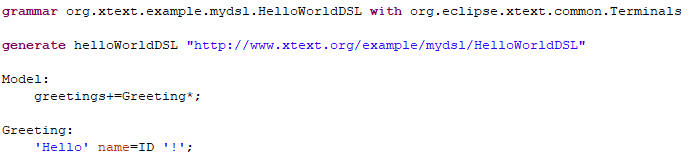
\includegraphics[width=\linewidth]{images/xtext/hello_world_xtext}
	\caption{Příklad zápisu gramatiky úrovně HelloWorld}
\end{figure}

Po vytvoření gramatiky je z ní nástroj Xtext schopný vygenerovat parser, textový editor a další infrastrukturu. Po vygenerování jsme schopni spustit instanci prostředí eclipse, která obsahuje plug-in s námi vytvořeným jazykem. Zde je již možné vytvořit nový projekt a v něm vytvořit soubory s příponou vytvořeného doménově specifického jazyka a je možné psát v jeho syntaxi. Prostředí samo hlídá dodržení syntaxe a vypisuje chyby, pokud syntaxe dodržena nebyla. Klávesovými zkratkami pro napovídání je možné editor vypisovat všechny možnosti, které je na základě syntaxe možné na dané místo psát. 

\begin{figure}[H]
	\centering
	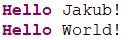
\includegraphics[width=0.2\linewidth]{images/xtext/hello_world_dsl}
	\caption{Syntaxe doménově specifického jazyka z gramatiky HelloWorld}
\end{figure}

Syntaxe psaní gramatiky v Xtextu není složitá a je možné se ji naučit v řádu desítek minut. Ukázka zápisu gramatiky bude přejata z návodu na příslušných internetových stránkách popsaných v sekci instalace. Na základě této gramatiky bude vytvořen soubor psaný v tomto doménově specifickém jazyce. Popis gramatiky musí začínat tzv. počátečním pravidlem. Obsahuje základní pravidla, která musí náš jazyk dodržovat. Toto pravidlo začíná návěštím, které si sami určíme. 

\begin{figure}[H]
	\centering
	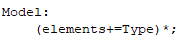
\includegraphics[width=0.4\linewidth]{images/xtext/model}
	\caption{Počáteční pravidlo}
\end{figure}

V tomto příkladě toto pravidlo vyjadřuje, že náš doménový model bude obsahovat libovolný počet ( \textit{*} ) elementů typu \textit{Type}, které jsou přidány do proměnné s názvem \textit{elements}.

\begin{figure}[H]
	\centering
	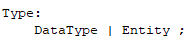
\includegraphics[width=0.4\linewidth]{images/xtext/type}
	\caption{pravidlo Type}
\end{figure}

Pravidlo typu \textit{Type} deleguje pravidlům \textit{DataType} nebo ( | ) pravidlu \textit{Entity}.

\begin{figure}[H]
	\centering
	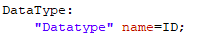
\includegraphics[width=0.4\linewidth]{images/xtext/dataType}
	\caption{pravidlo DataType}
\end{figure}

Pravidlo pro \textit{DataType} začíná klíčovým slovem \textit{Datatype}. Za ním následuje identifikátor, který je vyparsován z pravidla pro \textit{ID}, které je k nalezení v knihovně \textit{terminals}.

\begin{figure}[H]
	\centering
	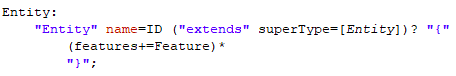
\includegraphics[width=0.8\linewidth]{images/xtext/entity}
	\caption{pravidlo Entity}
\end{figure}

Pravidlo pro \textit{Entity} opět začíná klíčovým slovem \textit{Entity} následováno názvem. Za ním následuje volitelné ( \textit{?} ) klíčové slovo \textit{extends}, které využívá typu \textit{superType} a přiřazuje mu proměnnou typu \textit{Entity}. Tímto způsobem je možné dědit různé typy stejně jako v objektově orientovaném programování.

\begin{figure}[H]
	\centering
	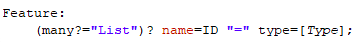
\includegraphics[width=0.7\linewidth]{images/xtext/feature}
	\caption{pravidlo Feature}
\end{figure}

Poslední pravidlo v našem příkladě je klíčové slovo \textit{many}, které je doporučené pro používání k popisu souboru více hodnot, s pojmenováním \textit{List}. Přiřazovací operátor ( \textit{?=} ) značí, že vlastnost \textit{many} je typu \textit{boolean}.

\begin{figure}[H]
	\centering
	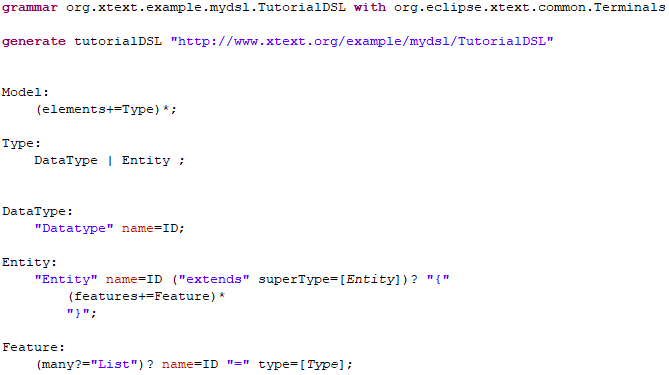
\includegraphics[width=\linewidth]{images/xtext/tutorial_xtext}
	\caption{kompletní zápis tvořené gramatiky}
\end{figure}

Z těchto příkladů je vidět několik nejzákladnějších syntaktických pravidel Xtextu. Klíčová slova jsou zapsána v uvozovkách. Jednoduché přiřazení je zapsáno pomocí ( \textit{=} ), zatímco přiřazení vícero hodnot je zapsáno jako ( \textit{+=} ) a přiřazení typu boolean zapsáno jako ( \textit{?=} ). Také je na příkladě vidět přiřazování kardinality elementům a to \textit{?} pro volitelné elementy, \textit{*} pro jakýkoliv počet elementů a \textit{+} pro jeden nebo více elementů.

Na základě této syntaxe jsme schopni vytvořit jednoduchý doménově specifický jazyk. Tato syntaxe byla použita pro zápis jednoduché databáze studentů. Data budou typu Int a String. První Entitou, která je v příkladě uvedena je entita \textit{StudentDatabase}, která má svůj název a více studentů. Každý student zapsán pomocí entity \textit{Student} má své jméno, ročník, ID, záznam o nějaké bakalářské nebo diplomové práci a list studovaných předmětů. Entita práce ( \textit{Thesis} ) má svůj název, počet stran a vícero zdrojů. Entita zdroj má svůj název, rok vydání a jméno autora. A jako poslední je popsána Entita předmět ( \textit{Subject} ), která má svůj název, jméno lektora a ročník, ve kterém je studován.

\begin{figure}[H]
	\centering
	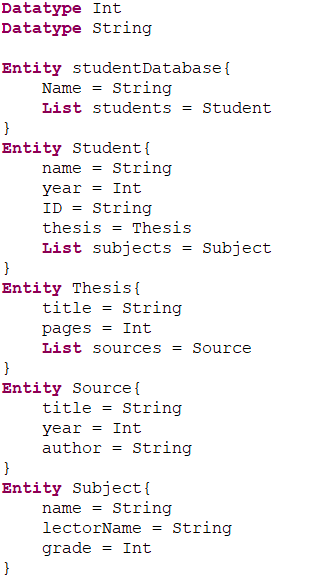
\includegraphics[width=0.5\linewidth]{images/xtext/tutorial_dsl}
	\caption{Doménově specifický jazyk psaný podle gramatiky}
\end{figure}

Nástroj Xtext obsahuje krom těchto syntaktických pravidel velké množství dalších funkcí a pravidel, pomocí kterých je možné vytvořit libovolně složitý jazyk. Tato pravidla jsou k nalezení v \cite{Xtext}.   

\subsection{TesaTK}

\textit{TesaTK} ( \textit{TE Software Assets Tool Kit} ) je doménově specifický jazyk vytvořený pomocí nástroje Xtext Danielem Mokošem ve společnosti ZF Engineering. Jazyk slouží k popisu a konfiguraci signálů, které se využívají v pozdějších konfigurátorech. Gramatika jazyka obsahuje desítky vlastností, které může výsledná konfigurace obsahovat. Zápis gramatiky obsahuje krom základních syntaktických pravidel i různé výčtové typy, konstanty a další. Pomocí tohoto jazyka je možné zapsat všechny možné varianty konfigurací na základě požadovaných vstupních a výstupních signálů, variant, požadovaných hardwarových komponent, systémů a subsystémů, pro které je konfigurace tvořena. 

Výhodou tohoto jazyka je hlavně kontrola správného zápisu konfigurace vývojovým prostředím Eclipse. Díky nástroji Xtext jsou při tvorbě konfigurace nabízeny možnosti, které je možné v konfiguraci zapsat a jsou hlídány syntaktické chyby, které by mohly mít velký dopad při aplikaci těchto konfigurací. Díky popisu konfigurace jako doménově specifického jazyka se specifickou syntaxí zůstávají všechny konfigurace v průběhu času jednotné a jsou tak uživatelsky přehlednější a jejich tvorba mnohem rychlejší. Při změně požadavků, nebo přidání vlastností, které jsou ke konfiguraci potřeba, stačí tyto změny zanést do gramatiky popsané v Xtextu a všechny konfigurace přepsat na základě těchto změn.

\section{Další nástroje}
V této části budou stručně popsány další nástroje, které slouží k tvorbě jazyků.

\subsection{textX}
Nástroj \textit{textX} je pythonový framework inspirovaný nástrojem Xtext. Nástroj nevyužívá \textit{EMF} jako Xtext, ale využívá metaprogramování Pythonu k reprezentaci tříd v paměti. Oproti Xtextu také nástroj textX negeneruje vývojové prostředí, ve kterém lze doménově specifický jazyk psát. Meta model je také možné vizualizovat pomocí nástroje \textit{GraphViz}. 

\subsection{Spoofax}
\textit{Spoofax} je další textový nástroj pro tvorbu jazyků. Stejně jako Xtext je distribuován jako zásuvný model vývojového prostředí Eclipse, ale je možné jej používat i ve vývojovém prostředí IntelliJ. Nástroj není komerční a je určen pro výzkum. Svou funkcionalitou připomíná nástroj Xtext. Stejně jako Xtext generuje vývojové prostředí, které je schopno s vytvořeným jazykem pracovat. 

\subsection{JetBrains MPS}
\textit{JetBrains MPS} je nástroj, který oproti ostatním zmíněným nástrojům není textový. Nástroj je především určený ke generování zdrojových kódů jazyků pro obecné použití. Využívá reprezentace zdrojových kódů v \textit{Abstraktním syntaktickém stomě} (z angl. \textit{Abstract syntax tree}) (AST). Každý uzel tohoto stromu reprezentuje určitou konstrukci v programovacím jazyce a může mít skupinu potomků a rodiče. Tento nástroj na základě tvorby a editace tohoto stromu generuje zdrojový kód a umožňuje tak vytvořit program netextovým přístupem, ale pomocí editace diagramů a tabulek. Tento nástroj také umožňuje jazyky rozšiřovat o nové funkce nebo vytvořit zcela nový jazyk.

\section{Shrnutí}
Pomocí nástroje Xtext jsme schopni jednoduše a rychle vytvořit vlastní doménově specifický jazyk a současně dostat vývojové prostředí, které bude vytvořený jazyk podporovat. Jazyk TesaTK je jazyk napsaný právě pomocí nástroje Xtext. Gramatika popsaná v nástroji obsahuje výčet vlastností a díky syntaxi gramatiky bude možné z gramatiky vytvořit model vlastností. Z tohoto modelu bude možné vytvořit varianty konfigurace a na základě těchto konfigurací bude možné generovat zdrojové kódy v jazyce tesa. Díky nástroji Xtext bude také možné tyto generované soubory kontrolovat a následně upravovat.




